% Created by: Hosein Hadipour
% Compilation is memory consuming. 
% Therefore, it is better to use the following command to compile: 
% latexmk -lualatex ./twinkleexample.tex

\documentclass[tikz]{standalone}
\usepackage{twinkle}
\usepackage{amsmath}

\begin{document}
\begin{tikzpicture}

\coordinate (here) at (0,0);

\drawRound{
\TFillCell[orange]{1}{2},
\BFillCell[purple]{2}{1},
\FillCellNew[orange]{0}{0}
}{
\TFillCell[orange]{1}{2},
\BFillCell[purple]{2}{1},
\FillCellNew[orange]{0}{0}
}{$\text{Round}~0$};

\drawRoundC{
\TFillCell[orange]{1}{2},
\BFillCell[purple]{2}{1},
\FillCellNew[orange]{0}{0}
}{
\TFillCell[orange]{1}{2},
\BFillCell[purple]{2}{1},
\FillCellNew[orange]{0}{0}
}{
\TFillCell[orange]{1}{2},
\BFillCell[purple]{2}{1},
\FillCellNew[orange]{0}{0}
}{
\TFillCell[orange]{1}{2},
}{
\TFillCell[orange]{1}{2},
}{$S$}{$R_0$}{$M$}{$R_1$};

\end{tikzpicture}
\end{document}
